\begin{myprops}
	\begin{itemize}
		\item Le symétrique d'une droite par rapport à une droite ou un point est une autre droite. La symétrie \hspace*{6cm}.
		\item Si deux droites sont \kw{symétriques par rapport à un point} alors elles sont \hspace*{4cm}.
	\end{itemize}
\end{myprops}

\begin{myexs}
	\begin{multicols}{2}
		\begin{center}
			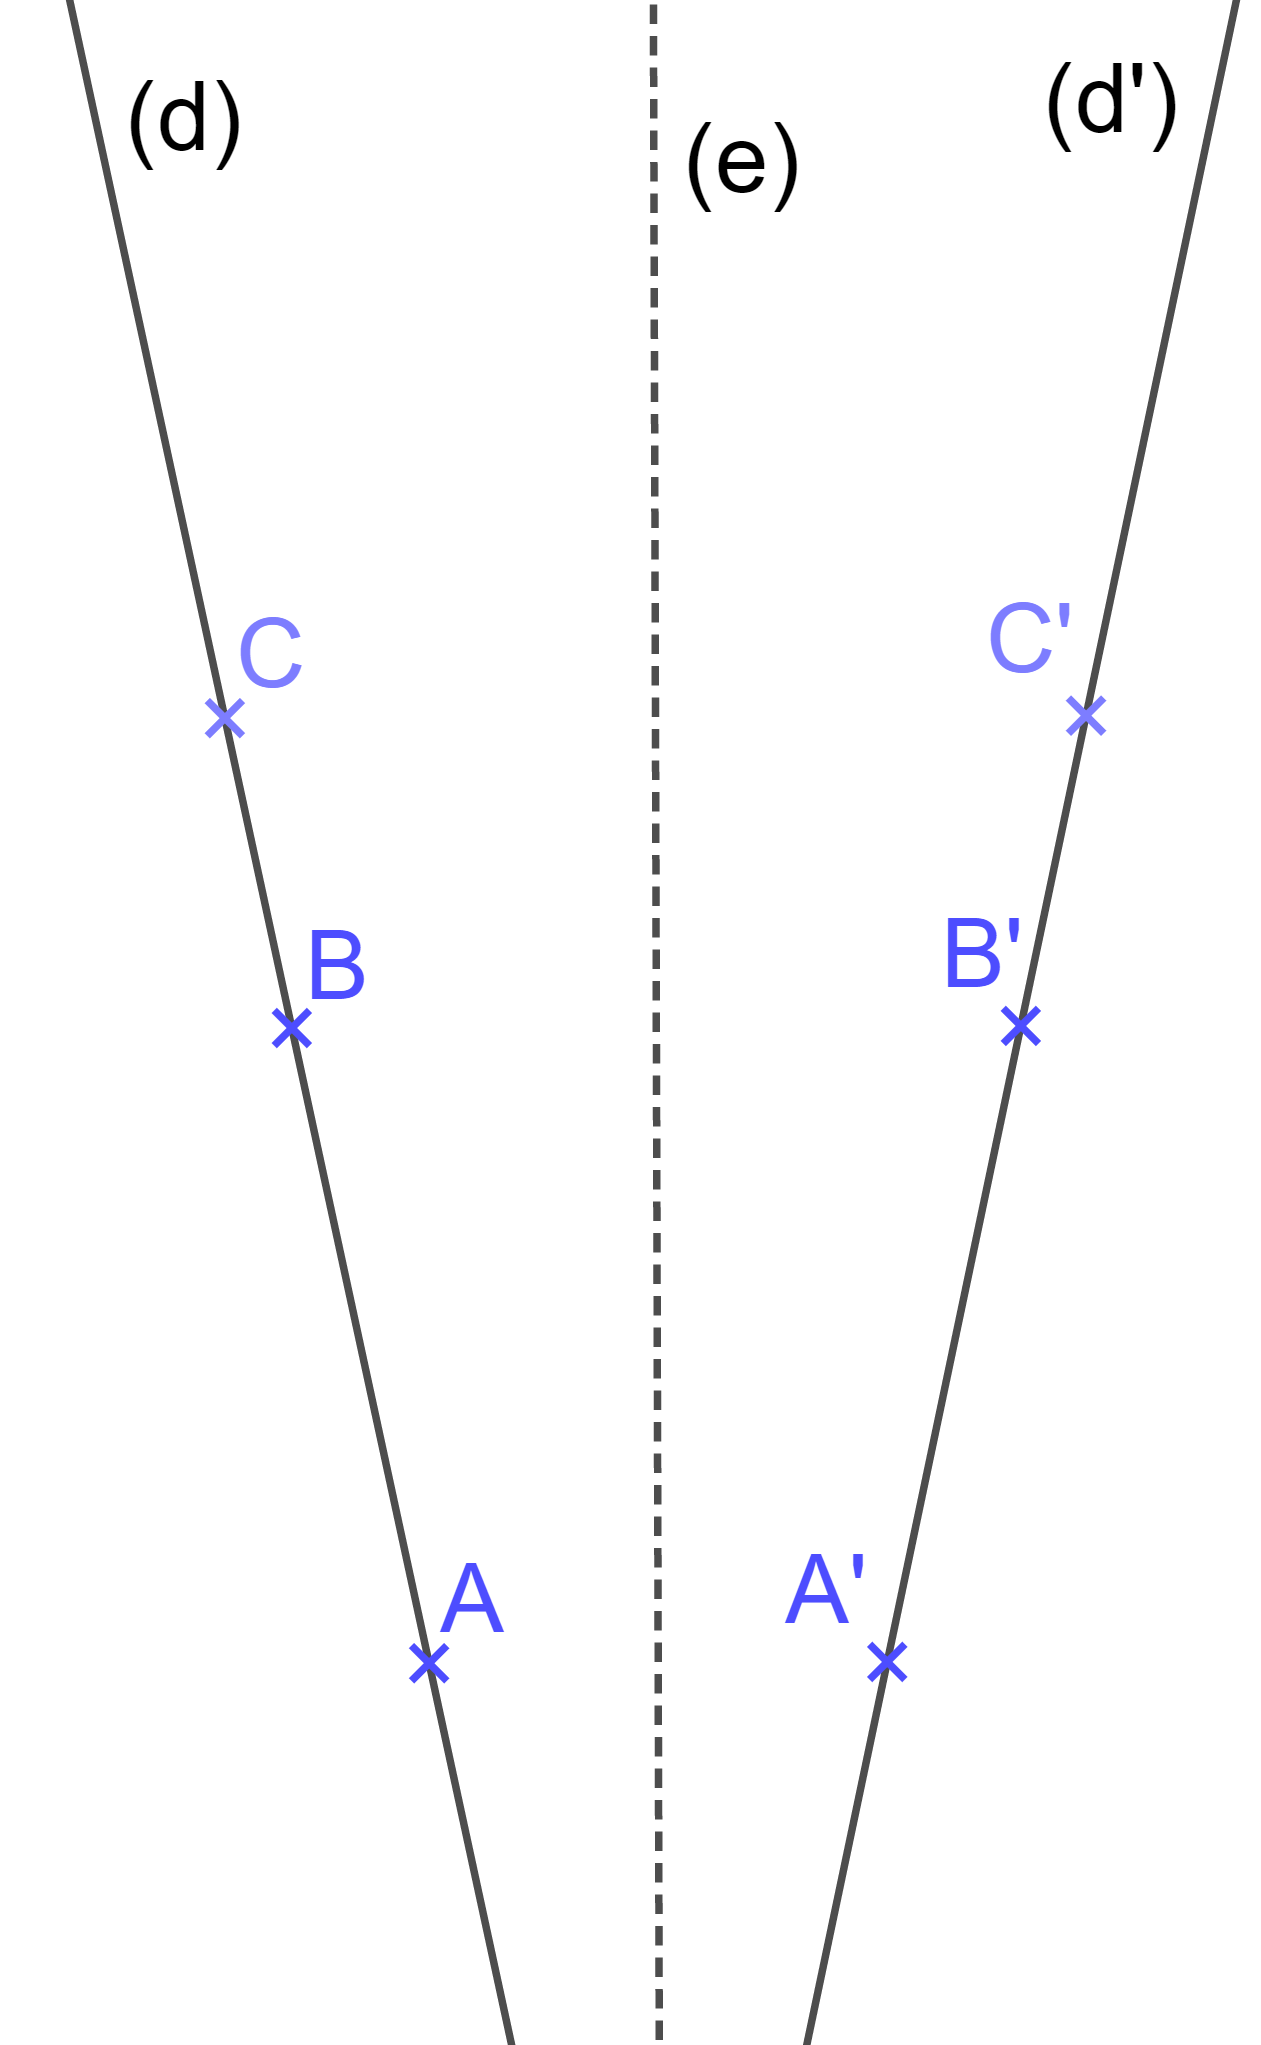
\includegraphics[scale=0.1]{sym_droites1}
		\end{center}

		\begin{itemize}
			\item Les points $A$, $B$ et $C$ sont alignés, donc $A'$, $B'$ et $C'$ leur symétriques par rapport à la droite $(e)$ sont \hspace*{6cm}
		\end{itemize}	
		
		\begin{center}
			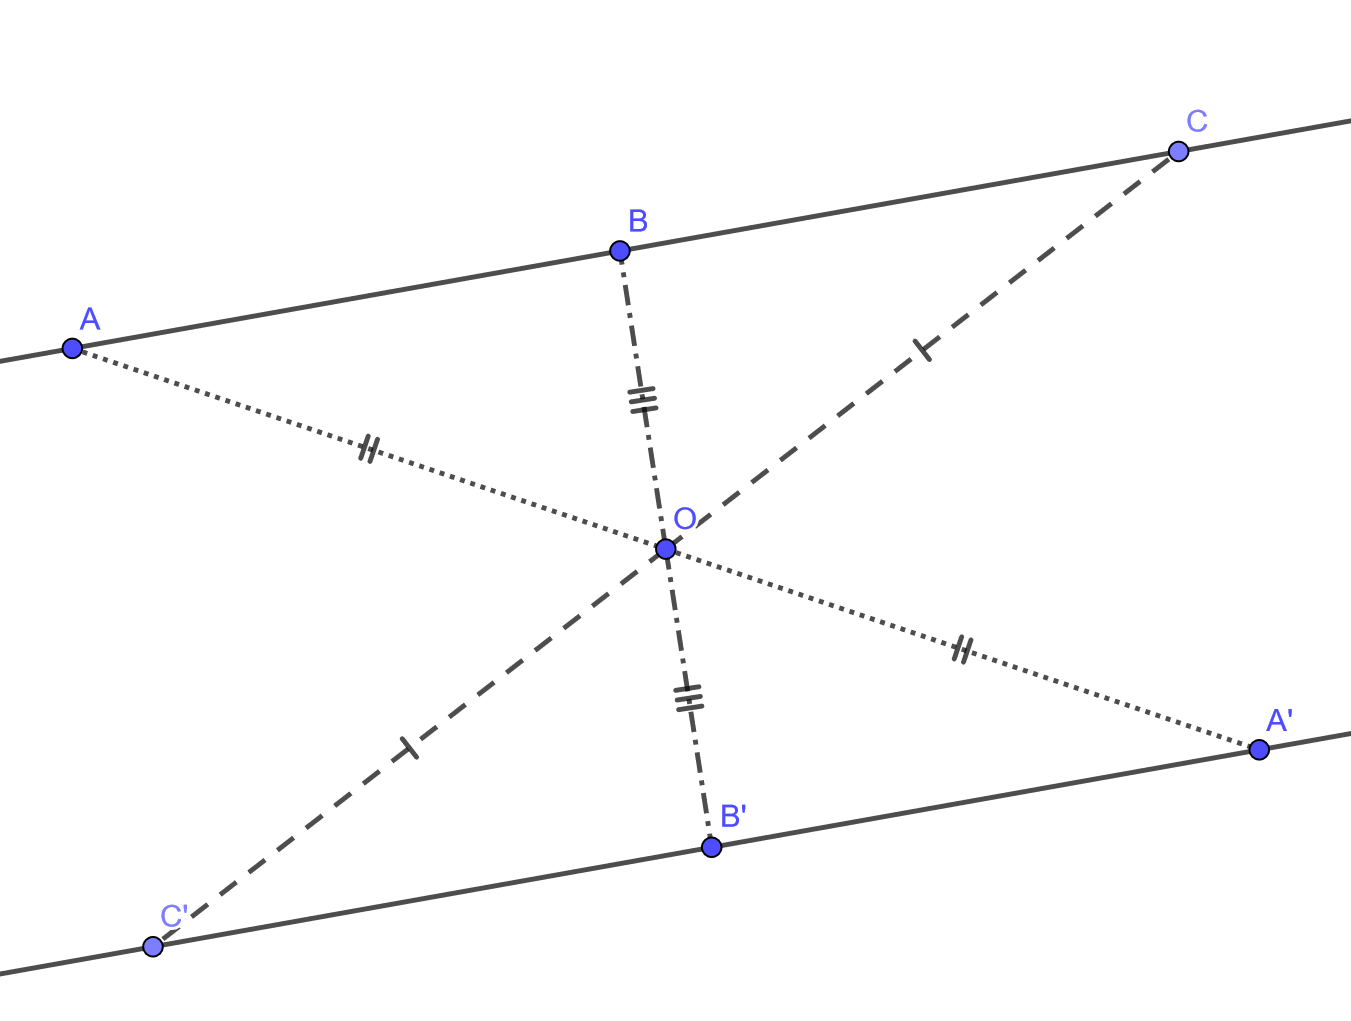
\includegraphics[scale=0.2]{sym_droites2}
		\end{center}
	
		\begin{itemize}
			\item Les points $A$, $B$ et $C$ sont alignés, donc $A'$, $B'$ et $C'$ leur symétriques par rapport à la droite $(e)$ sont \hspace*{6cm}.
			\item La droite $(AB)$ est \hspace*{4cm} \\ à la droite $(A'B')$.
		\end{itemize}
	\end{multicols}
\end{myexs}

\begin{myprop}
	Le symétrique d'un segment par rapport à une droite ou un point est un segment \hspace*{6cm} .
\end{myprop}

\begin{myex}
	\begin{center}
		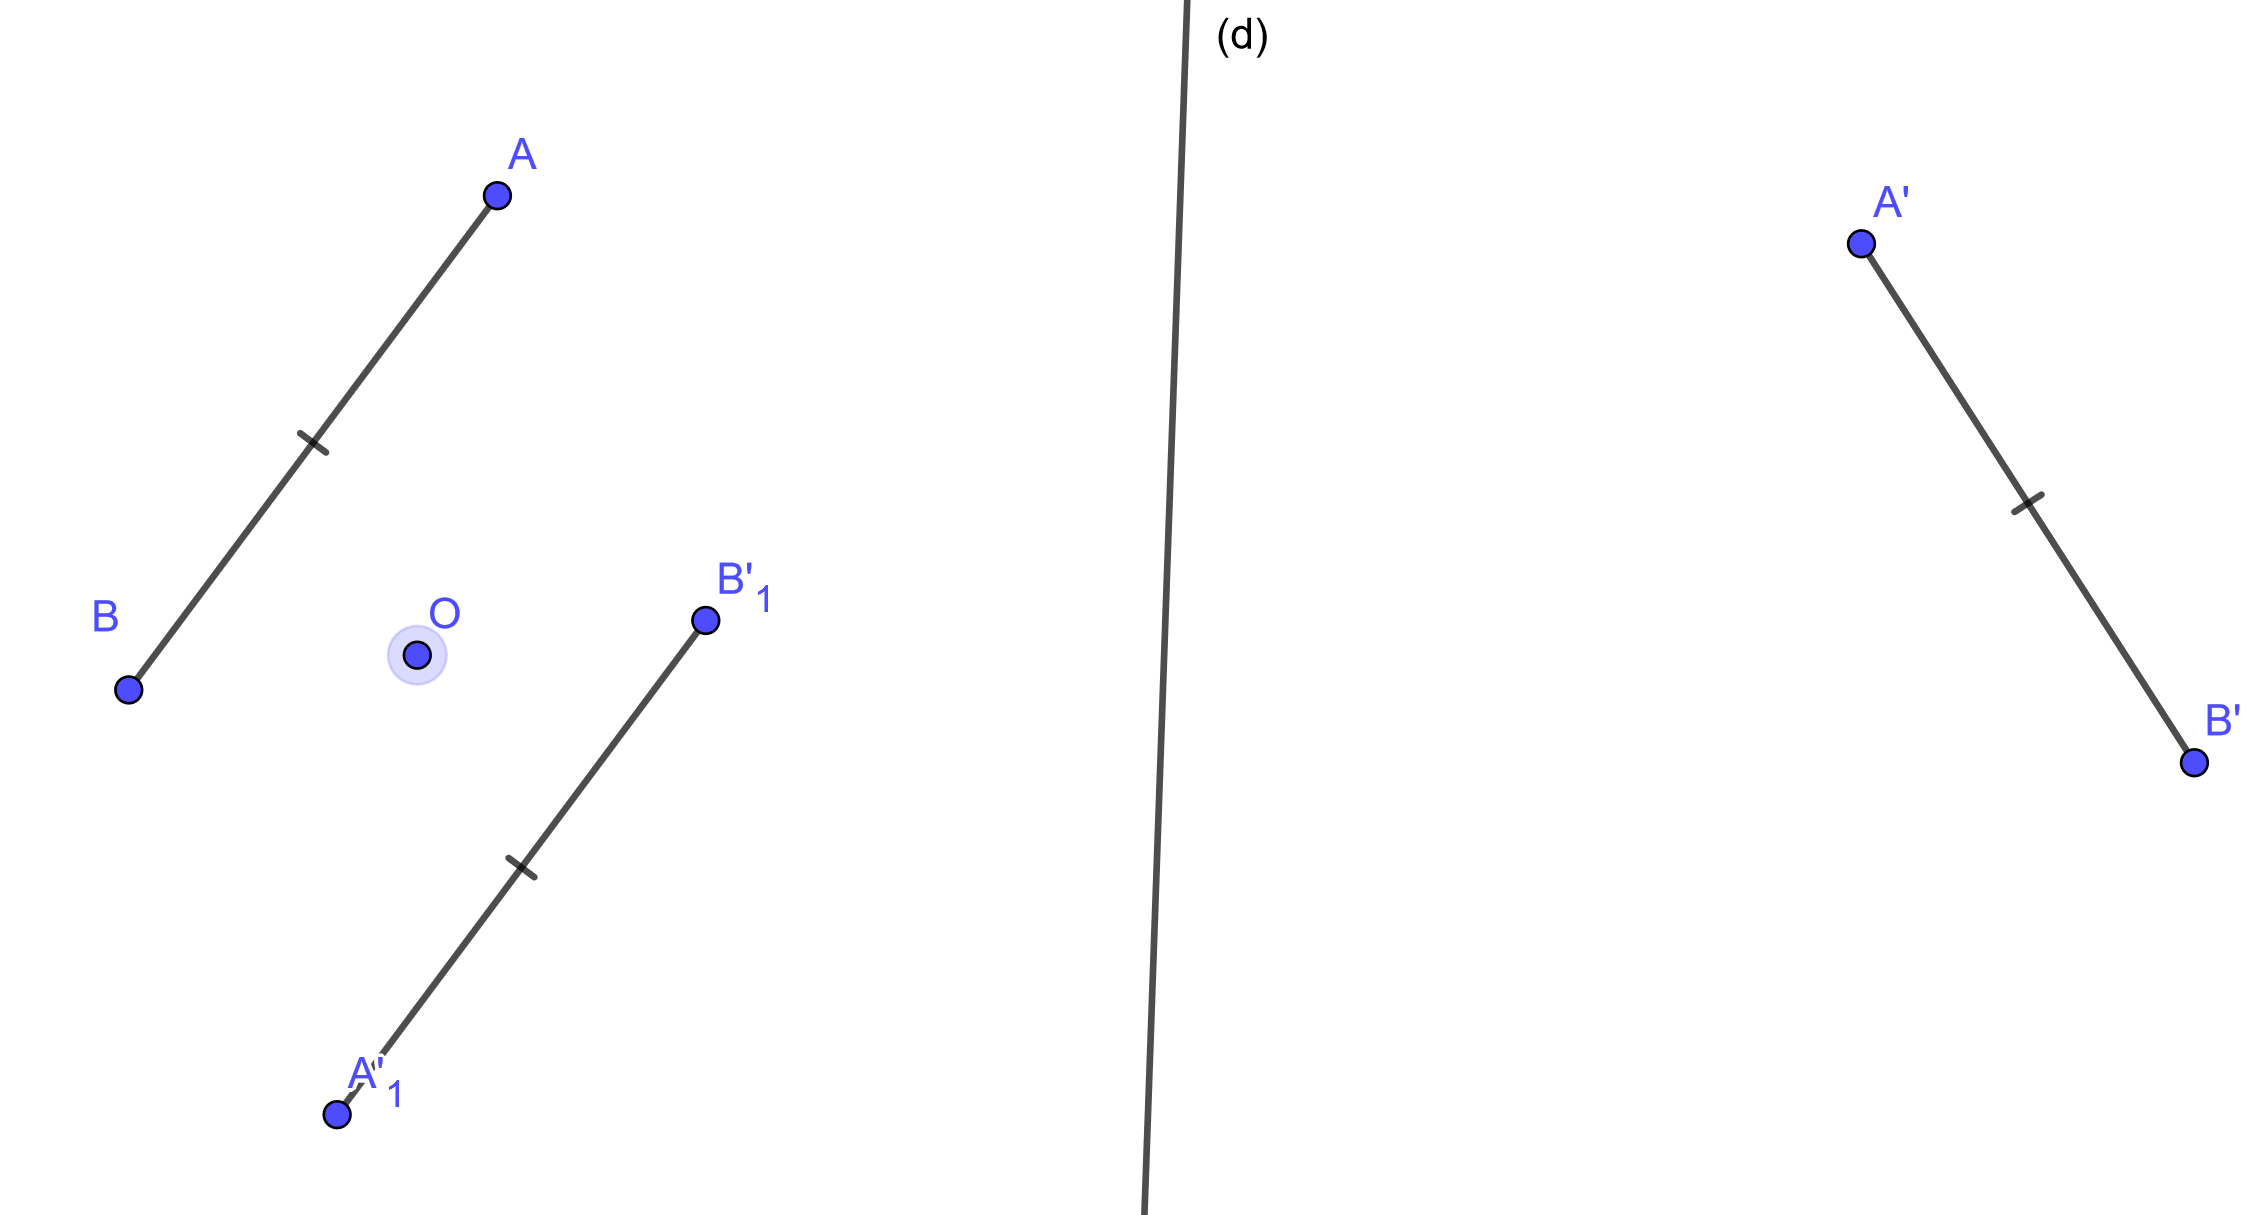
\includegraphics[scale=0.2]{sym_seg}
	\end{center}

Le segment $[A'B']$ est le symétrique du segment $[AB]$ par rapport à la droite $(d)$ et $[A'_1B'_1]$ le symétrique de $[AB]$ par rapport au point $O$. 
Ils ont tous \\

	
\end{myex}

\begin{myprop}
	Le symétrique d'une figure par rapport à une droite ou un point est une figure de même forme. La symétrie \kw{conserve \hspace*{8cm}} \\ .
\end{myprop}

\begin{myex}
	\begin{center}
		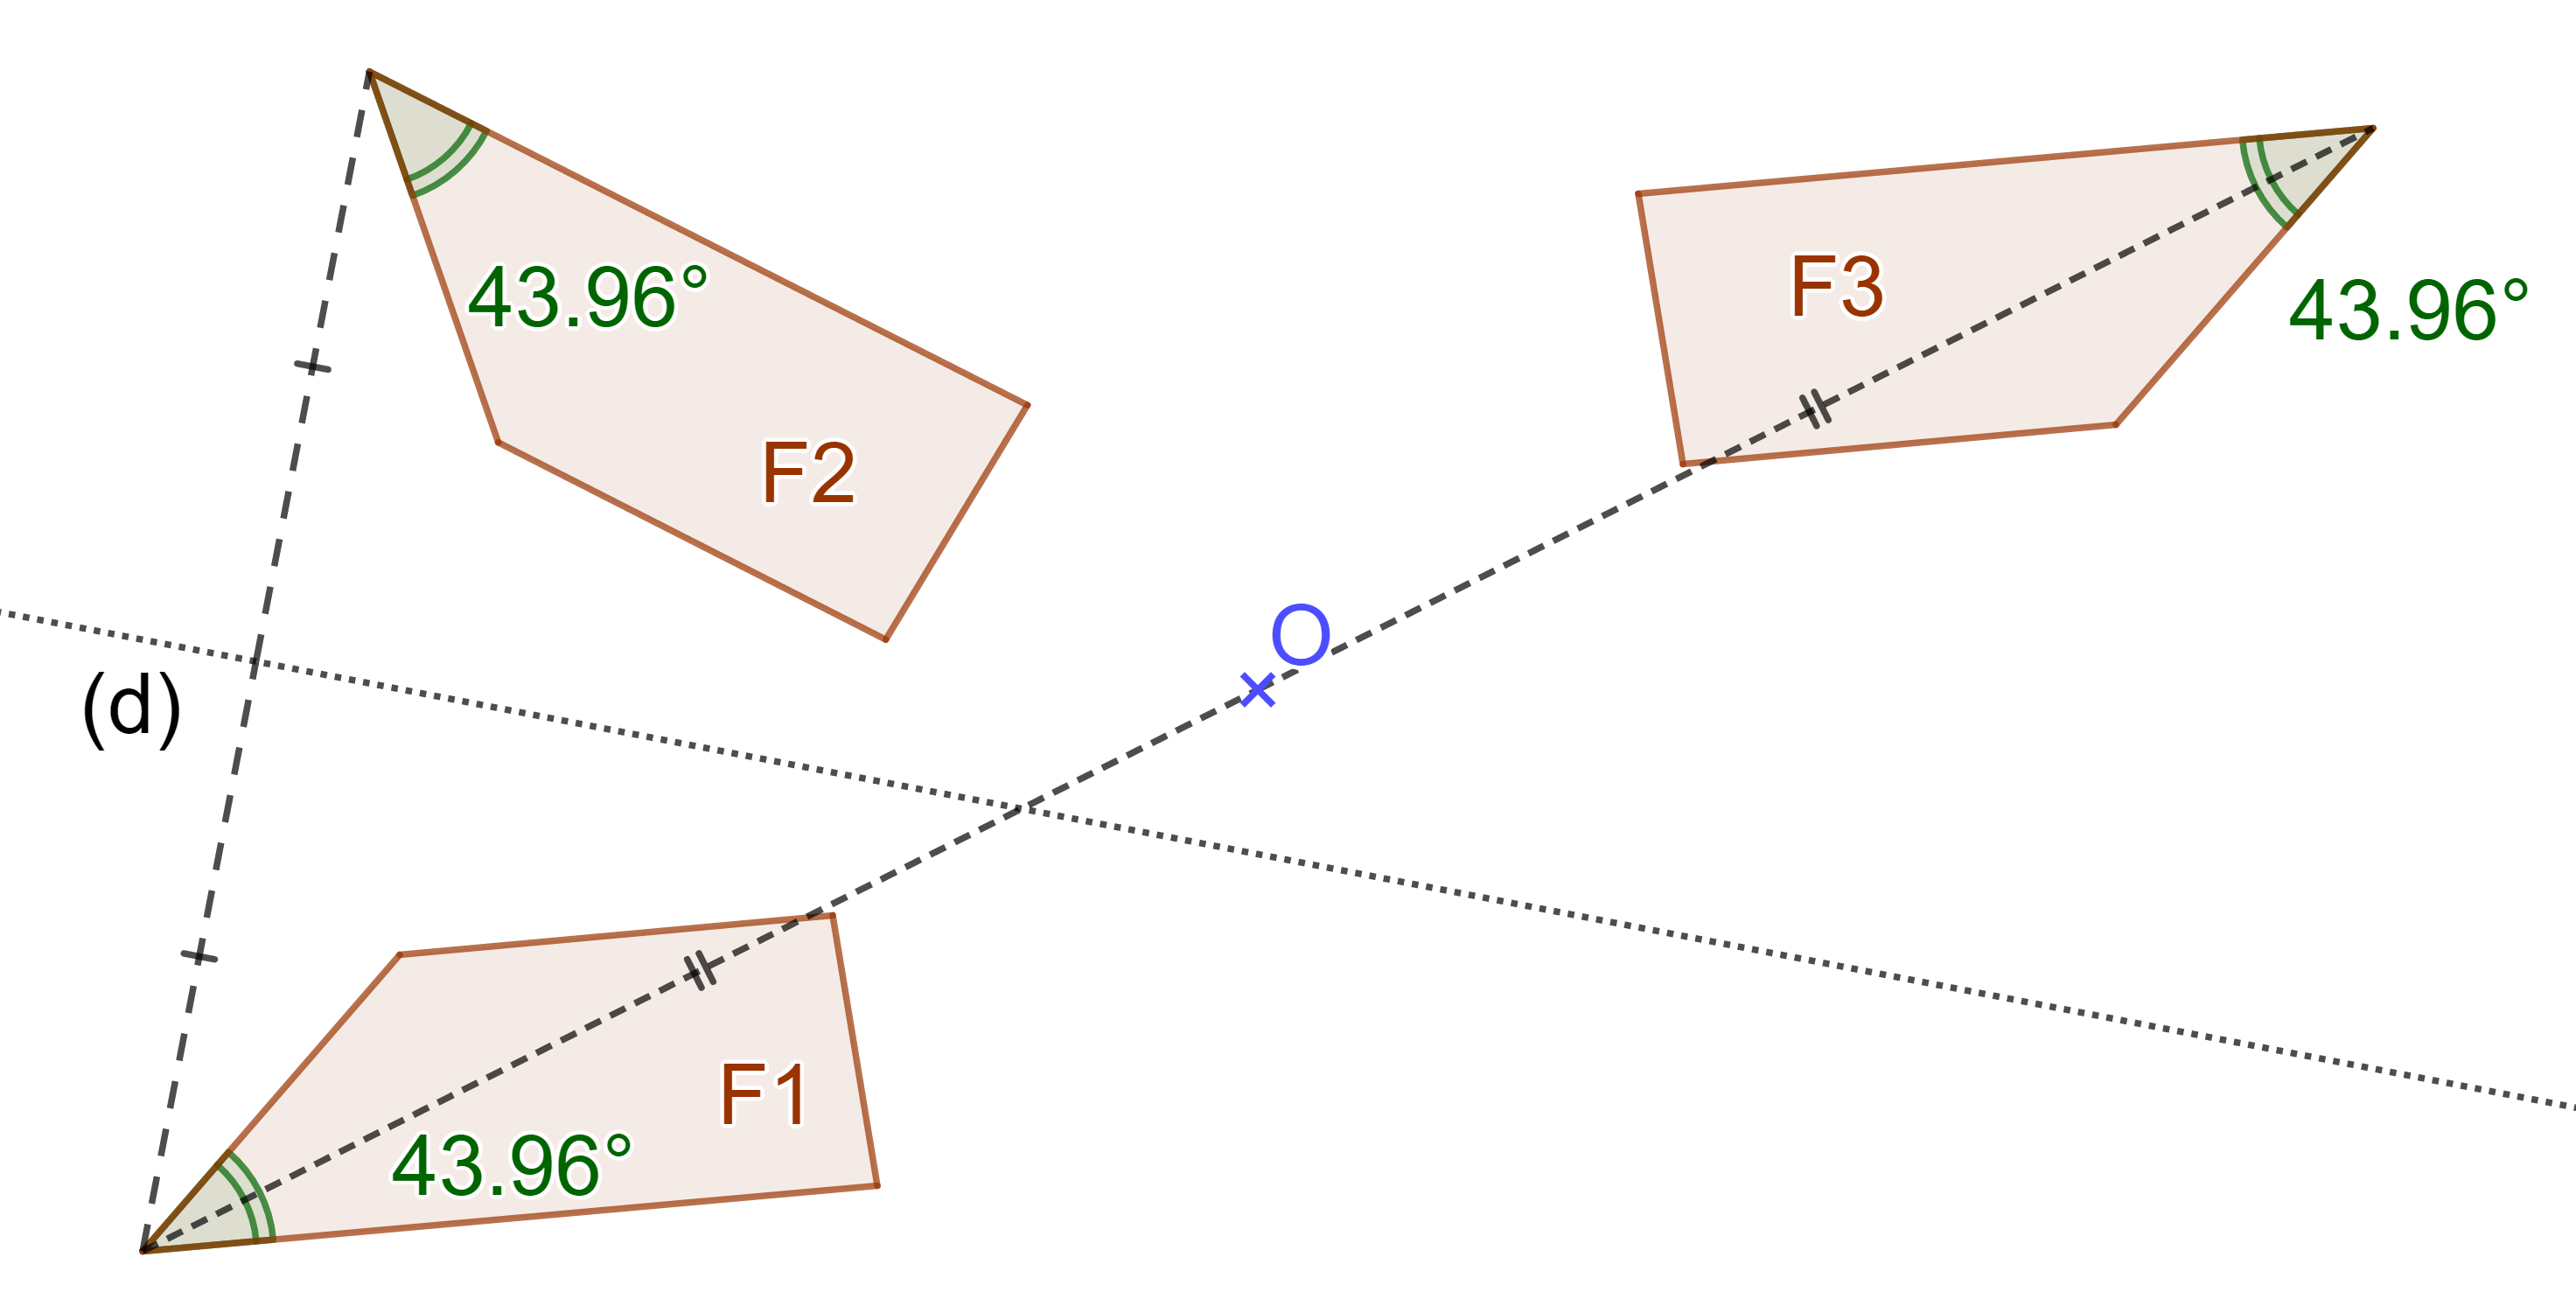
\includegraphics[scale=0.2]{sym_figures}
	\end{center}
	
	La figure $F2$ est le symétrique de $F1$ par rapport à la droite $(d)$; $F3$ est le symétrique de $F1$ par rapport au point O.
	Elles ont \\
\end{myex}

